\begin{figure}[t]
    \vspace{3mm}
    \centering
    
    \begin{subfigure}[t]{0.49\linewidth}
        \centering
        \begin{minipage}[t][0.8cm][t]{\linewidth}
            \centering\textbf{(a) Ring Placement}
        \end{minipage}
        \phantomsubcaption\label{fig:four_fingers}
        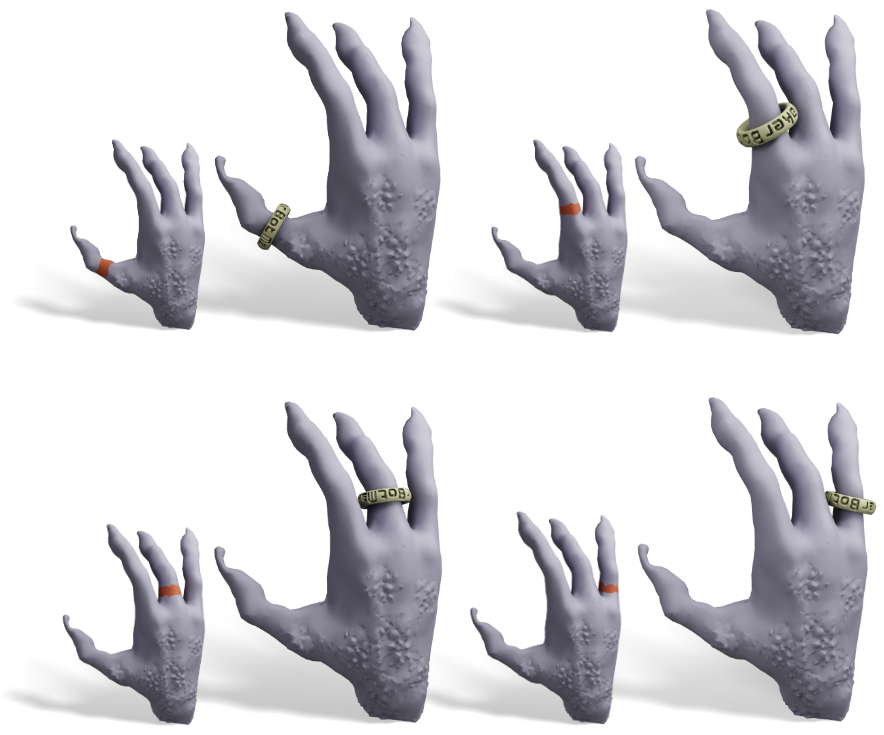
\includegraphics[width=\linewidth]{figures/region_control/four_fingers.png}
    \end{subfigure}
    \hfill
    \begin{subfigure}[t]{0.49\linewidth}
        \centering
        \begin{minipage}[t][0.8cm][t]{\linewidth}
            \centering\textbf{(b) Region Sensitivity}
        \end{minipage}
        \phantomsubcaption\label{fig:highlight-region}
        
\includegraphics[width=\linewidth]{figures/region_control/highlight-region-2-2.pdf}
    \end{subfigure}

    \vspace{3mm}
    \caption{
    \textbf{Region-controlled composition.}
    \textbf{(a)} Given four distinct user-selected target regions, \ourmethod{} places a ring precisely on each selected region, demonstrating explicit user control over the fitting process.
    \textbf{(b)} Because the method adheres strictly to the selected region, asset placement is sensitive to the region definition; for example, glasses sit naturally on the ears only if a small portion of the ear region is included in the selection.
    }
    \label{fig:region_control}
\end{figure}